\section{Player Engagement}
\label{chap:player_engagement}



\subsection{Questionnaire}



\begin{table}[H]
    \centering
    \begin{tabularx}{\textwidth}{|c|X|c|c|c|c|c|}
        \hline
        & \multicolumn{1}{c|}{\textbf{Statements}}  & \multicolumn{1}{c|}{\textbf{Disagree}} & \multicolumn{1}{c|}{\textbf{Neutral}}  & \multicolumn{1}{c|}{\textbf{Agree}} & \multicolumn{1}{c|}{\textbf{Avg S}} & \multicolumn{1}{c|}{\textbf{Avg C}}\\ \hline
        \textbf{S1} & I was curious about the medals I could achieve during the game. & 47.4\% & 26.3\% & 26.3\% & 2.67 & 3.14 \\
        \textbf{S2} & I got new medals and awards during the entire test period. & 26.3\% & 21.1\% & 52.7\% & 3.25 & 3.43 \\
        \textbf{S3} & The game gave me enough challenges. & 57.9\% & 36.8\% & 5.3\% & 2.17 & 2.86 \\
        \textbf{S4} & Challenges between friends inspired me to use the app more. & 31.6\% & 10.5\% & 57.9\% & 2.92 & 4.14 \\
        \textbf{S5} & I often gave reactions to other players' activities and achievements. & 57.9\% & 21.1\% & 21.1\% & 2.50 & 2.00 \\
        \textbf{S6} & Notifications made sure I used the application more. & 26.3\% & 26.3\% & 47.3\% & 3.08 & 3.43 \\
        \hline
    \end{tabularx}
    \caption{Results from the statements related to engagement.}
    \label{tab:statements_engagemet_answers}
    \vspace*{-\baselineskip}
\end{table}



\begin{figure}[H]
    \centering
    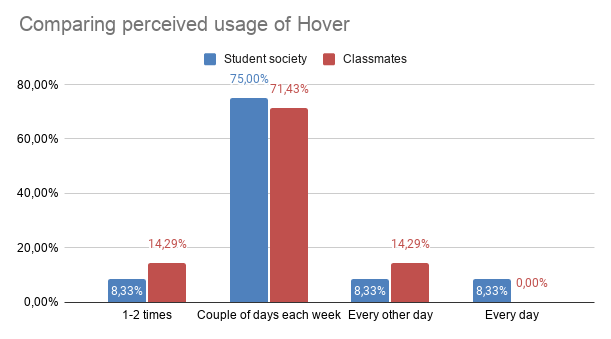
\includegraphics[width=\textwidth]{Images/Results/Engagement/PerceivedUsageOfTheApp.png}
    \caption{The perceived usage of Hover is relatively equal between the two groups. }
    \label{fig:engagement_perceived_usage}
\end{figure}


\begin{table}[H]
    \centering
    \begin{tabularx}{\textwidth}{|c|X|c|c|c|c|}
        \hline
        & \multicolumn{1}{c|}{\textbf{Questions}}  & \multicolumn{1}{c|}{\textbf{Avg S}} & \multicolumn{1}{c|}{\textbf{Avg C}}  & \multicolumn{1}{c|}{\textbf{All}} & \\ \hline
        \textbf{Q11} & On average, how long (number of minutes) did you use Hover every day during the test period? & 5.73 & 4.29 & 5.2 & minutes \\
        \textbf{Q12} & How many times during the test period did you accept a challenge from friends? & 1.25 & 1.43 & 1.32 & times \\
        \textbf{Q13} & How many times during the test period did you challenge friends? & 0.42 & 0.43 & 0.42 & times \\
        \textbf{Q14} & On average, how many reactions did you give per day during the test period? & 2.23 & 0.59 & 1.63 & reaction \\
        \hline
    \end{tabularx}
   \caption{The participants’ responses to the questions in the questionnaire regarding their engagement.}
    \label{tab:engagement_questions}
    \vspace*{-\baselineskip}
\end{table}









\subsection{Application Usage Data}


\begin{figure}[H]
    \centering
    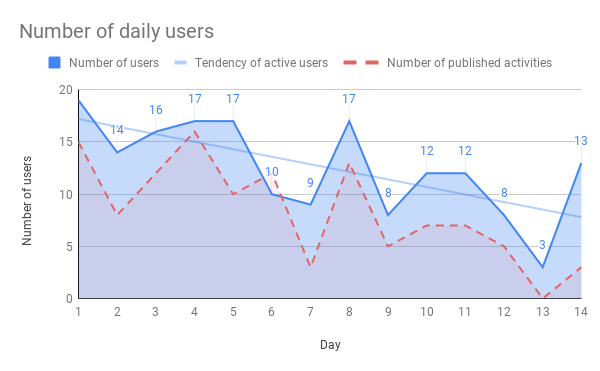
\includegraphics[width=\textwidth]{Images/Results/Engagement/NumberOfDailyUsers.png}
    \caption{The number of daily users during the 14 days of testing. }
    \label{fig:engagement_daily_users}
\end{figure}

\begin{figure}[H]
    \centering
    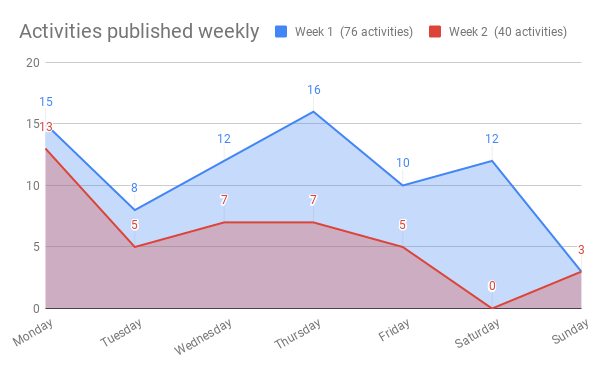
\includegraphics[width=\textwidth]{Images/Results/Engagement/ActivitiesPublishedWeekly.png}
    \caption{A comparison of the activity level between the two weeks. }
\label{fig:engagement_actvities_weekly}
\end{figure}


\begin{figure}[H]
    \centering
    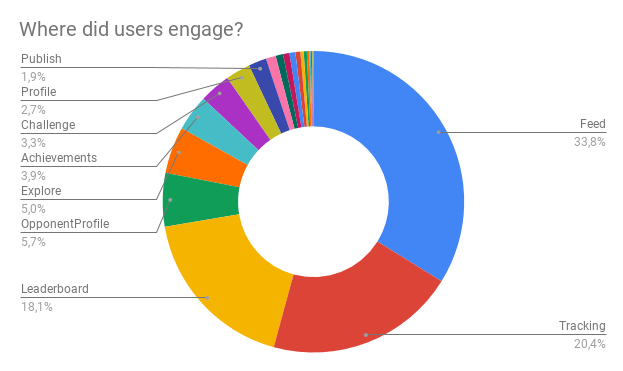
\includegraphics[width=\textwidth]{Images/Results/Engagement/WhereDidUsersEngage.png}
    \caption{A pie chart of the most used screens.}
    \label{fig:engagement_screens}
\end{figure}

\begin{figure}[H]
    \centering
    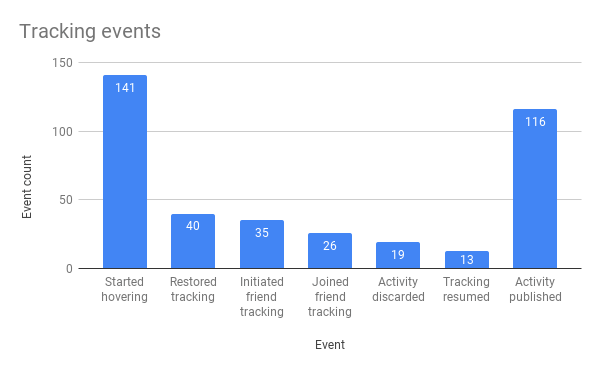
\includegraphics[width=\textwidth]{Images/Results/Engagement/TrackingEvents.png}
    \caption{The tracking events recorded by Google Analytics.}
    \label{fig:engagement_tracking_events}
\end{figure}

\begin{figure}[H]
    \centering
    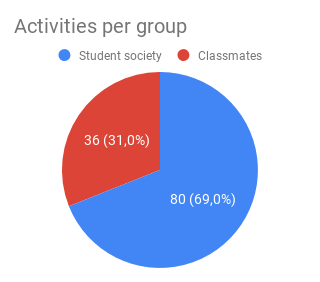
\includegraphics[width=0.6\textwidth]{Images/Results/Engagement/ActivitiesPerGroup.png}
    \caption{A pie chart showing the number of activities published by the two groups.}
    \label{fig:engagement_actvities_per_group}
\end{figure}

\begin{figure}[H]
    \centering
    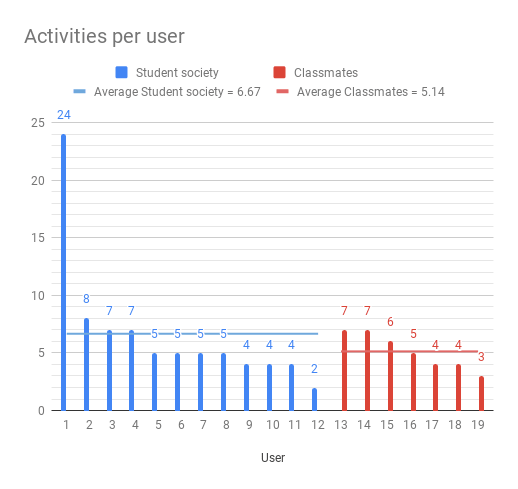
\includegraphics[width=\textwidth]{Images/Results/Engagement/ActivitiesPerUser.png}
    \caption{A bar chart showing the number of activities published by each participant.}
    \label{fig:engagement_actvities_per_user}
\end{figure}



\begin{table}[H]
    \centering
    \begin{tabularx}{\textwidth}{|X|c|c|c|}
        \hline
        & \multicolumn{1}{c|}{\textbf{Student society}}  & \multicolumn{1}{c|}{\textbf{Classmates}} & \multicolumn{1}{c|}{\textbf{Combined}} \\ \hline
        Number of activities utilizing friend tracking & 32/80 & 11/36 & 43/116 \\
        Percentage of activities using friend tracking & 40.0\% & 30.6\% & 37.1\% \\
        Number of participants using it at least once & 10/12 & 4/7 & 14/19 \\
        Average use per participant & 2.67 & 1.57 & 2.26 \\
        \hline
    \end{tabularx}
    \caption{Numbers describing the participants’ use of Hover’s friend tracking feature.}
    \label{tab:engagement_friend_tracking}
    \vspace*{-\baselineskip}
\end{table}


\begin{figure}[H]
    \centering
    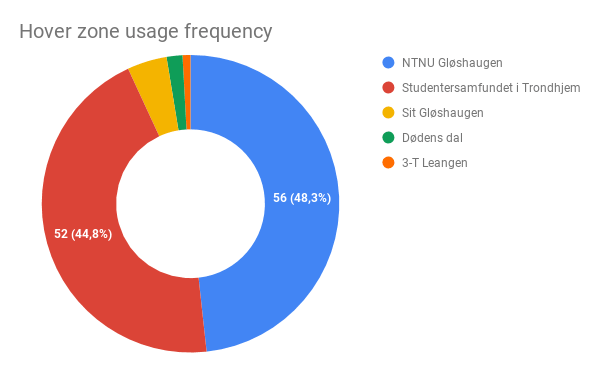
\includegraphics[width=0.8\textwidth]{Images/Results/Engagement/HoverZoneFrequency.png}
    \caption{The hover zones used.}
    \label{fig:engagement_hover_zones}
\end{figure}

\begin{figure}[H]
    \centering
    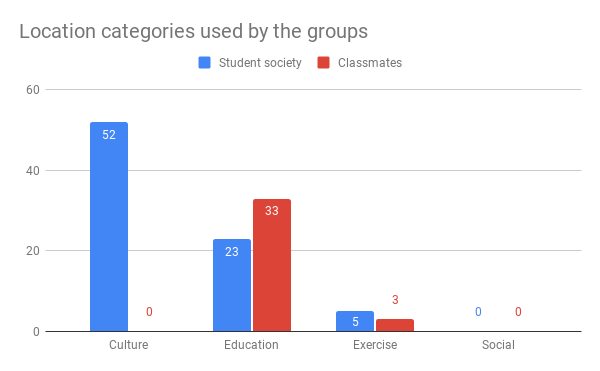
\includegraphics[width=\textwidth]{Images/Results/Engagement/LocationCategoriesUsed.png}
    \caption{The difference in what location categories the groups used.}
    \label{fig:engagement_categories_used}
\end{figure}

\begin{figure}[H]
    \centering
    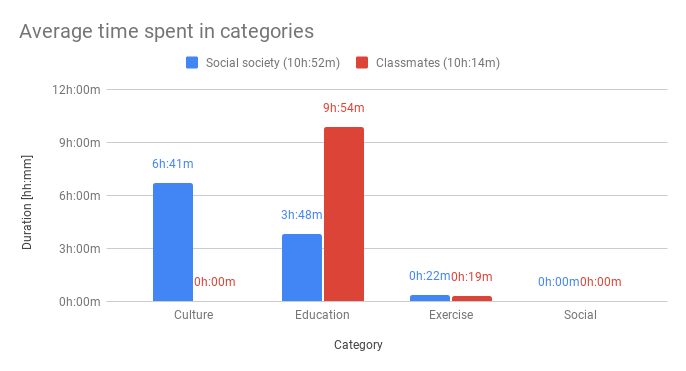
\includegraphics[width=\textwidth]{Images/Results/Engagement/AverageDurationInCategories.png}
    \caption{ A bar chart of the average time spent hovering in the four categories.}
    \label{fig:engagement_ duration_in_category}
\end{figure}

\begin{figure}[H]
    \centering
    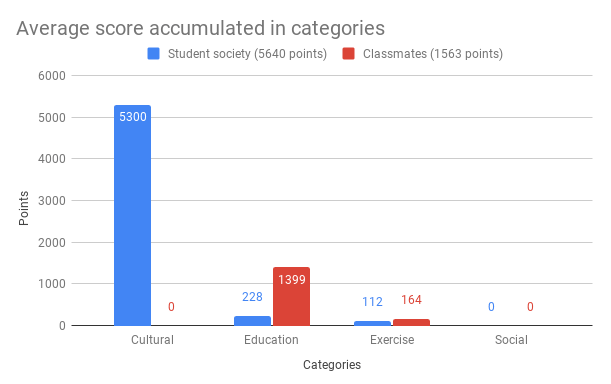
\includegraphics[width=\textwidth]{Images/Results/Engagement/AverageScoreInCategories.png}
    \caption{A bar chart of the average score for the two groups in each category.}
    \label{fig:engagement_points_in category}
\end{figure}


\begin{figure}[H]
    \centering
    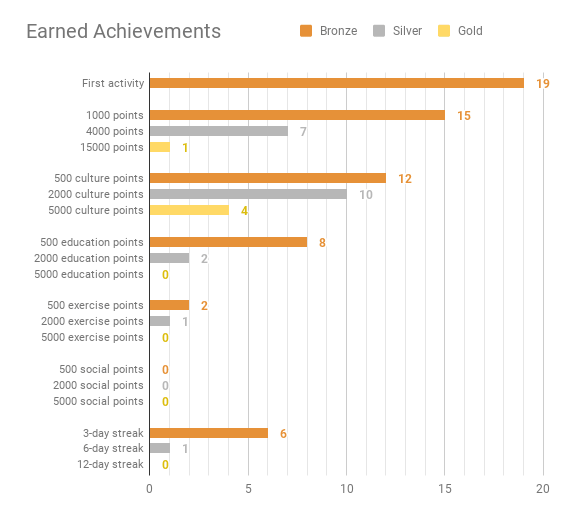
\includegraphics[width=\textwidth]{Images/Results/Engagement/EarnedAchievements.png}
    \caption{A bar chart showing the number and types of achievements earned.}
    \label{fig:engagement_achievement_earned}
\end{figure}


\begin{figure}[H]
    \centering
    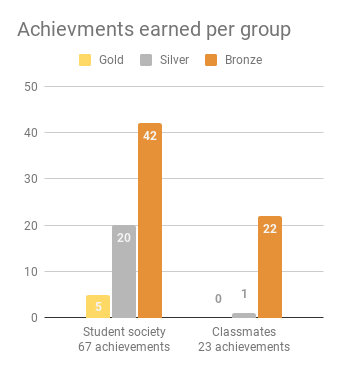
\includegraphics[width=0.7\textwidth]{Images/Results/Engagement/AchievmentsEarnedPerGroup.png}
    \caption{A bar chart showing the number of achievements earned by the two groups.}
    \label{fig:engagement_achievement_per_group}
\end{figure}


\begin{figure}[H]
    \centering
    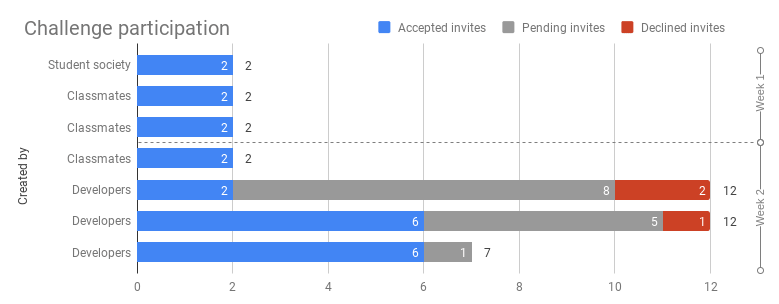
\includegraphics[width=\textwidth]{Images/Results/Engagement/ChallengeParticipation.png}
    \caption{A stacked bar chart showing the number of participants for each challenge.}
    \label{fig:engagement_created_challenges}

\end{figure}


\begin{figure}[H]
    \centering
    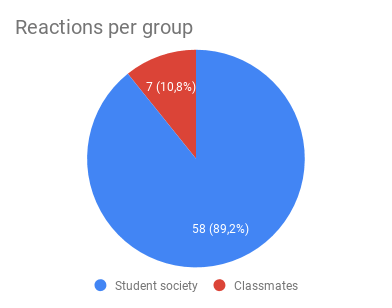
\includegraphics[width=0.6\textwidth]{Images/Results/Engagement/ReactionsPerGroup.png}
    \caption{A pie chart showing the difference in reactions given by the two groups .}
    \label{fig:engagement_reactions_per_group}
\end{figure}


\begin{figure}[H]
    \centering
    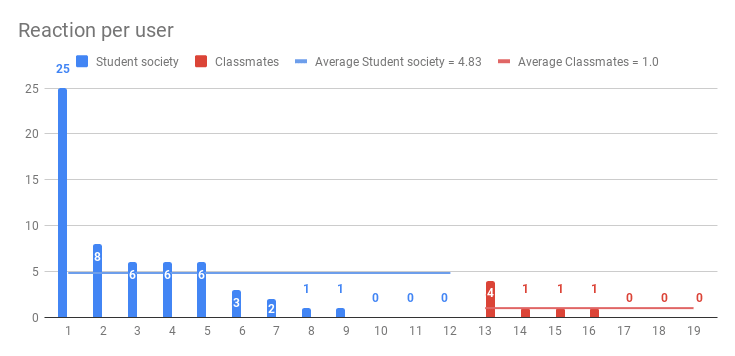
\includegraphics[width=\textwidth]{Images/Results/Engagement/ReactionsPerUser.png}
    \caption{A bar chart showing the number of reactions given by each user.}
    \label{fig:engagement_reactions_per_user}
\end{figure}

\subsection{Summary}